\documentclass[14pt]{extbook}
\usepackage{multicol, enumerate, enumitem, hyperref, color, soul, setspace, parskip, fancyhdr} %General Packages
\usepackage{amssymb, amsthm, amsmath, bbm, latexsym, units, mathtools} %Math Packages
\everymath{\displaystyle} %All math in Display Style
% Packages with additional options
\usepackage[headsep=0.5cm,headheight=12pt, left=1 in,right= 1 in,top= 1 in,bottom= 1 in]{geometry}
\usepackage[usenames,dvipsnames]{xcolor}
\usepackage{dashrule}  % Package to use the command below to create lines between items
\newcommand{\litem}[1]{\item#1\hspace*{-1cm}\rule{\textwidth}{0.4pt}}
\pagestyle{fancy}
\lhead{Progress Quiz 4}
\chead{}
\rhead{Version A}
\lfoot{4378-7085}
\cfoot{}
\rfoot{Fall 2020}
\begin{document}

\begin{enumerate}
\litem{
Solve the quadratic equation below. Then, choose the intervals that the solutions belong to, with $x_1 \leq x_2$ (if they exist).\[ 15x^{2} +14 x + 2 = 0 \]\begin{enumerate}[label=\Alph*.]
\item \( x_1 \in [-2.5, -0.6] \text{ and } x_2 \in [-1.6, 0.4] \)
\item \( x_1 \in [-9.5, -9] \text{ and } x_2 \in [7.9, 8.4] \)
\item \( x_1 \in [-0.6, 1.5] \text{ and } x_2 \in [0.2, 1.7] \)
\item \( x_1 \in [-13.1, -9.2] \text{ and } x_2 \in [-3.9, -2.5] \)
\item \( \text{There are no Real solutions.} \)

\end{enumerate} }
\litem{
Write the equation of the graph presented below in the form $f(x)=ax^2+bx+c$, assuming  $a=1$ or $a=-1$. Then, choose the intervals that $a, b,$ and $c$ belong to.
\begin{center}
    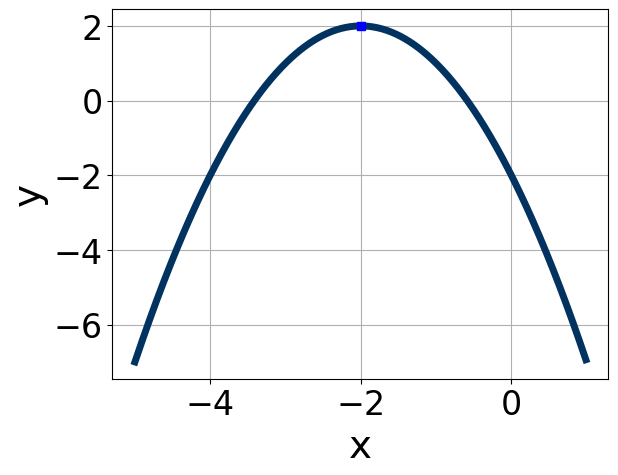
\includegraphics[width=0.5\textwidth]{../Figures/quadraticGraphToEquationCopyA.png}
\end{center}
\begin{enumerate}[label=\Alph*.]
\item \( a \in [-2, 0], \hspace*{5mm} b \in [3, 11], \text{ and } \hspace*{5mm} c \in [-28, -23] \)
\item \( a \in [0, 2], \hspace*{5mm} b \in [3, 11], \text{ and } \hspace*{5mm} c \in [4, 7] \)
\item \( a \in [0, 2], \hspace*{5mm} b \in [-9, -5], \text{ and } \hspace*{5mm} c \in [25, 28] \)
\item \( a \in [-2, 0], \hspace*{5mm} b \in [-9, -5], \text{ and } \hspace*{5mm} c \in [-28, -23] \)
\item \( a \in [0, 2], \hspace*{5mm} b \in [-9, -5], \text{ and } \hspace*{5mm} c \in [4, 7] \)

\end{enumerate} }
\litem{
Solve the quadratic equation below. Then, choose the intervals that the solutions $x_1$ and $x_2$ belong to, with $x_1 \leq x_2$.\[ 10x^{2} +33 x -54 = 0 \]\begin{enumerate}[label=\Alph*.]
\item \( x_1 \in [-1.5, 4.5] \text{ and } x_2 \in [3.16, 4.52] \)
\item \( x_1 \in [-46, -44] \text{ and } x_2 \in [11.84, 12.08] \)
\item \( x_1 \in [-5.5, -2.5] \text{ and } x_2 \in [0.97, 1.48] \)
\item \( x_1 \in [-12, -8] \text{ and } x_2 \in [0.5, 0.69] \)
\item \( x_1 \in [-14.5, -10.5] \text{ and } x_2 \in [0.25, 0.55] \)

\end{enumerate} }
\litem{
Factor the quadratic below. Then, choose the intervals that contain the constants in the form $(ax+b)(cx+d); b \leq d.$\[ 36x^{2} -60 x + 25 \]\begin{enumerate}[label=\Alph*.]
\item \( a \in [11.54, 12.85], \hspace*{5mm} b \in [-8, 1], \hspace*{5mm} c \in [1.54, 3.75], \text{ and } \hspace*{5mm} d \in [-8, 1] \)
\item \( a \in [1.91, 2.42], \hspace*{5mm} b \in [-8, 1], \hspace*{5mm} c \in [17.99, 18.19], \text{ and } \hspace*{5mm} d \in [-8, 1] \)
\item \( a \in [5.18, 6.28], \hspace*{5mm} b \in [-8, 1], \hspace*{5mm} c \in [4.63, 6.26], \text{ and } \hspace*{5mm} d \in [-8, 1] \)
\item \( a \in [-0.08, 1.61], \hspace*{5mm} b \in [-31, -25], \hspace*{5mm} c \in [0.66, 1.26], \text{ and } \hspace*{5mm} d \in [-32, -26] \)
\item \( \text{None of the above.} \)

\end{enumerate} }
\litem{
Solve the quadratic equation below. Then, choose the intervals that the solutions belong to, with $x_1 \leq x_2$ (if they exist).\[ 12x^{2} +13 x -7 = 0 \]\begin{enumerate}[label=\Alph*.]
\item \( x_1 \in [-23.17, -23] \text{ and } x_2 \in [20.6, 23.4] \)
\item \( x_1 \in [-0.45, 0.37] \text{ and } x_2 \in [0.8, 2.2] \)
\item \( x_1 \in [-2.27, -0.78] \text{ and } x_2 \in [-0.1, 0.6] \)
\item \( x_1 \in [-18.34, -17.61] \text{ and } x_2 \in [3.7, 5.5] \)
\item \( \text{There are no Real solutions.} \)

\end{enumerate} }
\litem{
Write the equation of the graph presented below in the form $f(x)=ax^2+bx+c$, assuming  $a=1$ or $a=-1$. Then, choose the intervals that $a, b,$ and $c$ belong to.
\begin{center}
    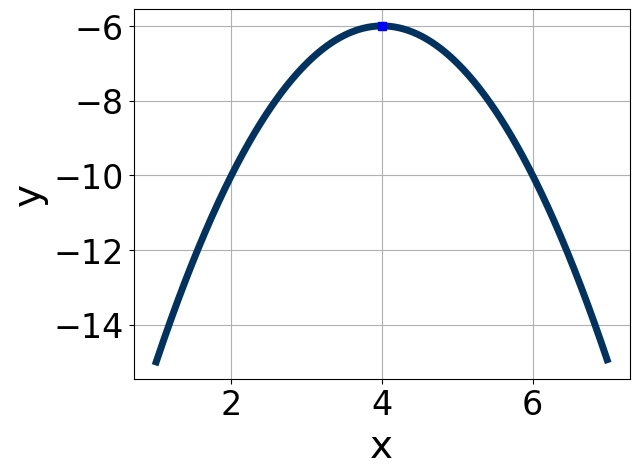
\includegraphics[width=0.5\textwidth]{../Figures/quadraticGraphToEquationA.png}
\end{center}
\begin{enumerate}[label=\Alph*.]
\item \( a \in [-5, 0], \hspace*{5mm} b \in [-10, -5], \text{ and } \hspace*{5mm} c \in [-16, -10] \)
\item \( a \in [0, 3], \hspace*{5mm} b \in [6, 11], \text{ and } \hspace*{5mm} c \in [20, 25] \)
\item \( a \in [0, 3], \hspace*{5mm} b \in [6, 11], \text{ and } \hspace*{5mm} c \in [8, 14] \)
\item \( a \in [-5, 0], \hspace*{5mm} b \in [6, 11], \text{ and } \hspace*{5mm} c \in [-16, -10] \)
\item \( a \in [0, 3], \hspace*{5mm} b \in [-10, -5], \text{ and } \hspace*{5mm} c \in [20, 25] \)

\end{enumerate} }
\litem{
Graph the equation below.\[ f(x) = -(x-3)^2 - 17 \]\begin{enumerate}[label=\Alph*.]
\begin{multicols}{2}\item 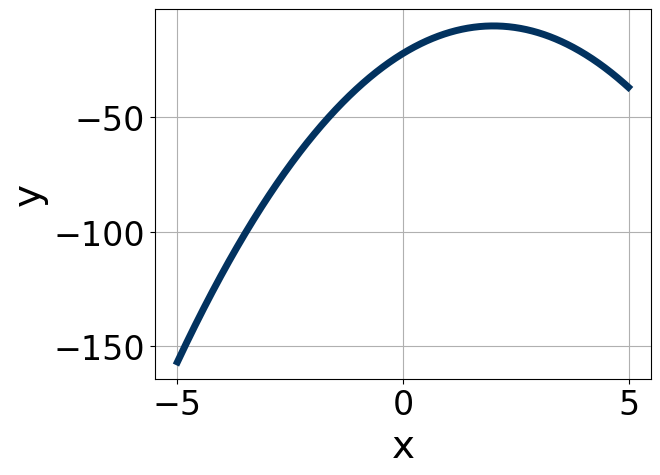
\includegraphics[width = 0.3\textwidth]{../Figures/quadraticEquationToGraphCopyAA.png}\item 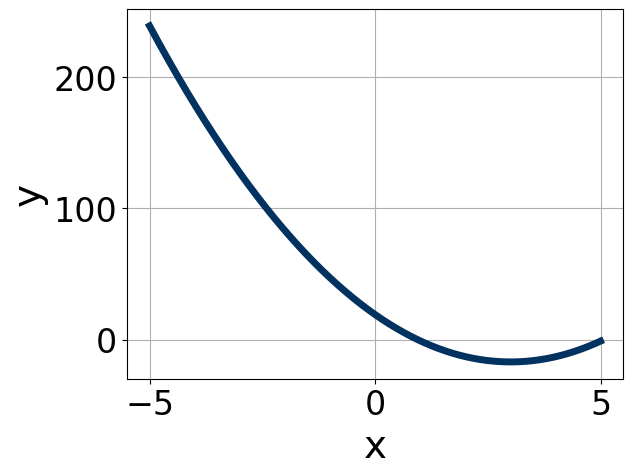
\includegraphics[width = 0.3\textwidth]{../Figures/quadraticEquationToGraphCopyBA.png}\item 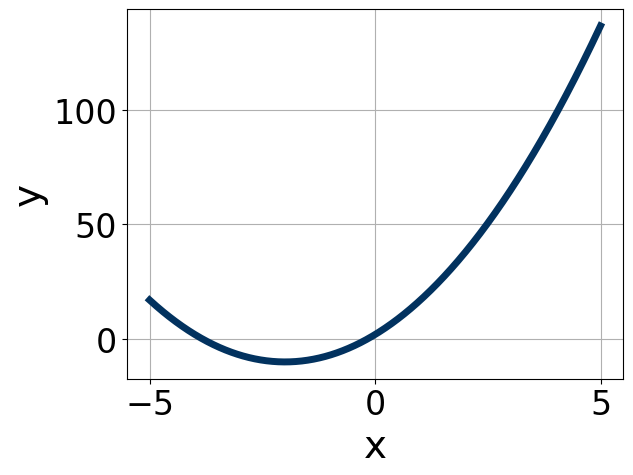
\includegraphics[width = 0.3\textwidth]{../Figures/quadraticEquationToGraphCopyCA.png}\item 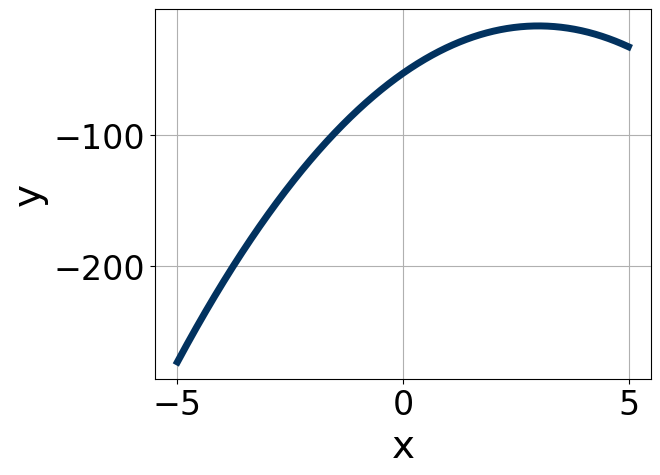
\includegraphics[width = 0.3\textwidth]{../Figures/quadraticEquationToGraphCopyDA.png}\end{multicols}\item None of the above.
\end{enumerate} }
\litem{
Solve the quadratic equation below. Then, choose the intervals that the solutions $x_1$ and $x_2$ belong to, with $x_1 \leq x_2$.\[ 25x^{2} +60 x + 36 = 0 \]\begin{enumerate}[label=\Alph*.]
\item \( x_1 \in [-7.82, -3.87] \text{ and } x_2 \in [-0.32, -0.22] \)
\item \( x_1 \in [-30.29, -29.97] \text{ and } x_2 \in [-30.01, -29.83] \)
\item \( x_1 \in [-3.99, -2.42] \text{ and } x_2 \in [-0.49, -0.39] \)
\item \( x_1 \in [-1.95, -0.24] \text{ and } x_2 \in [-1.32, -1.01] \)
\item \( x_1 \in [-2.86, -1.53] \text{ and } x_2 \in [-0.67, -0.54] \)

\end{enumerate} }
\litem{
Graph the equation below.\[ f(x) = -(x-3)^2 - 19 \]\begin{enumerate}[label=\Alph*.]
\begin{multicols}{2}\item 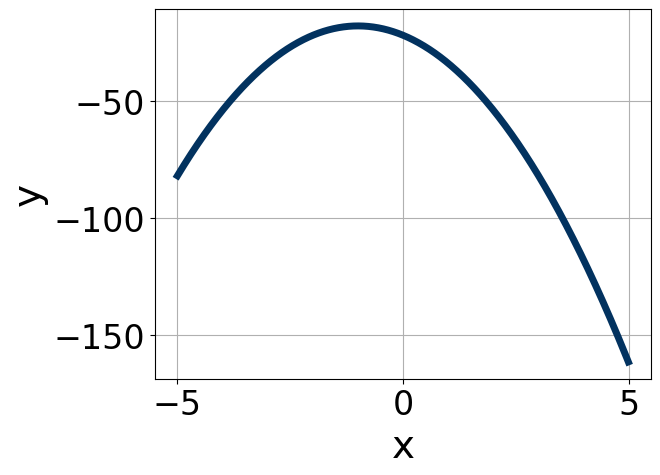
\includegraphics[width = 0.3\textwidth]{../Figures/quadraticEquationToGraphAA.png}\item 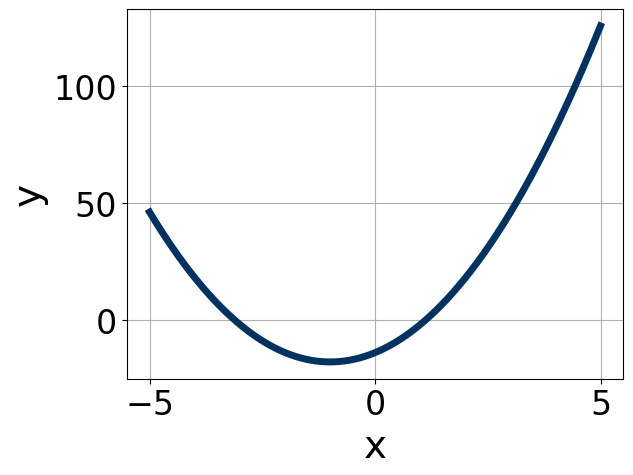
\includegraphics[width = 0.3\textwidth]{../Figures/quadraticEquationToGraphBA.png}\item 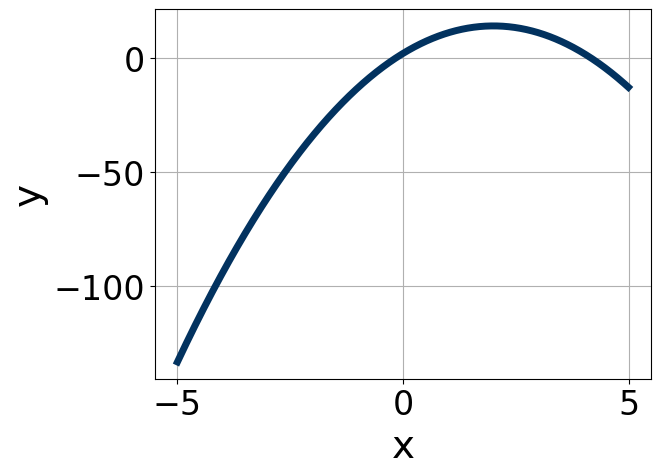
\includegraphics[width = 0.3\textwidth]{../Figures/quadraticEquationToGraphCA.png}\item 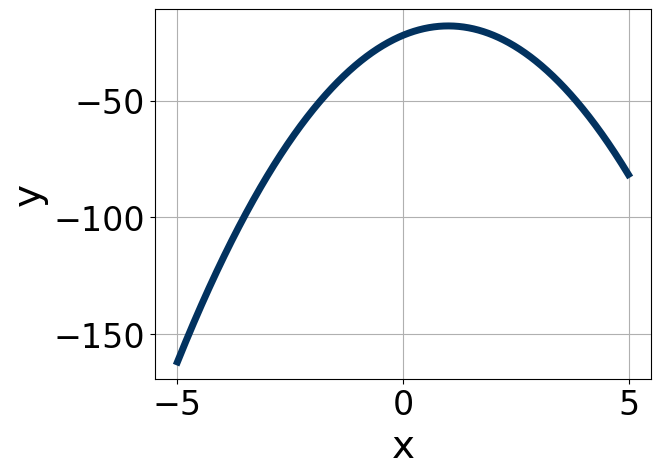
\includegraphics[width = 0.3\textwidth]{../Figures/quadraticEquationToGraphDA.png}\end{multicols}\item None of the above.
\end{enumerate} }
\litem{
Factor the quadratic below. Then, choose the intervals that contain the constants in the form $(ax+b)(cx+d); b \leq d.$\[ 54x^{2} +33 x -10 \]\begin{enumerate}[label=\Alph*.]
\item \( a \in [1.2, 4.7], \hspace*{5mm} b \in [-8, 6], \hspace*{5mm} c \in [17.76, 19.31], \text{ and } \hspace*{5mm} d \in [3, 7] \)
\item \( a \in [-1.6, 1.9], \hspace*{5mm} b \in [-15, -10], \hspace*{5mm} c \in [0.73, 1.12], \text{ and } \hspace*{5mm} d \in [42, 49] \)
\item \( a \in [7.7, 11.3], \hspace*{5mm} b \in [-8, 6], \hspace*{5mm} c \in [5.22, 6.9], \text{ and } \hspace*{5mm} d \in [3, 7] \)
\item \( a \in [22.5, 27.2], \hspace*{5mm} b \in [-8, 6], \hspace*{5mm} c \in [1.84, 2.68], \text{ and } \hspace*{5mm} d \in [3, 7] \)
\item \( \text{None of the above.} \)

\end{enumerate} }
\end{enumerate}

\end{document}